\documentclass[journal=jpcbfk,manuscript=article,layout=traditional]{achemso}

\usepackage{amsmath,amssymb}
\usepackage{siunitx}
\usepackage{booktabs}
% generated by qbscreen/make_numbers_tex.py — do not edit by hand
\newcommand{\tContactMin}{109}
\newcommand{\tContactMax}{290}
\newcommand{\tContactGeo}{160}
\newcommand{\betaMin}{2.5}
\newcommand{\betaMax}{3.4}
\newcommand{\nScanPoints}{33}
\newcommand{\lamFlHalf}{0.20}
\newcommand{\lamMethyl}{0.63}
\newcommand{\lamBenzyl}{0.48}
\newcommand{\lamAla}{0.92}
\newcommand{\aNfiveDFT}{441}
\newcommand{\aNtenDFT}{165}
\newcommand{\partnerMAO}{257}
\newcommand{\partnerDAO}{58}
\newcommand{\DeltaMaxMin}{0.53}
\newcommand{\DeltaMaxMax}{0.93}
\newcommand{\tauCompMax}{\ensuremath{3.9\times10^{-11}}}
\newcommand{\tauCompMin}{\ensuremath{1.1\times10^{-13}}}
\newcommand{\JCompMin}{\ensuremath{2.9\times10^{5}}}
\newcommand{\JCompMax}{\ensuremath{5.6\times10^{7}}}
\newcommand{\JtauInverted}{57}
\newcommand{\JtauActless}{0.18}
\newcommand{\DMAO}{-1817}
\newcommand{\DDAO}{-1217}
\newcommand{\capMAO}{\ensuremath{5.0\times10^{-5}}}
\newcommand{\capDAO}{\ensuremath{9.3\times10^{-6}}}
\newcommand{\tAnchor}{22}
\newcommand{\tAnchorWb}{4}
\newcommand{\partnerCapMin}{\ensuremath{3.6\times10^{-8}}}
\newcommand{\partnerCapMax}{\ensuremath{8.8\times10^{-5}}}
\newcommand{\spinOneRatio}{2.0}
\newcommand{\DMAOspin}{-914}
\newcommand{\DDAOspin}{-674}
\newcommand{\capMAOspin}{\ensuremath{4.3\times10^{-4}}}
\newcommand{\capDAOspin}{\ensuremath{4.1\times10^{-4}}}
\newcommand{\DCRY}{-11.4}
\newcommand{\cryNinetyMin}{0.21}
\newcommand{\cryNinetyMax}{1.74}
\newcommand{\cryPowderMin}{0.18}
\newcommand{\cryPowderMax}{1.42}


\author{Hikaru Wakaura}
\altaffiliation{ORCID: 0000-0001-8381-8323}
\email{h.wakaura@qiri.co.jp}
\affiliation{QIRI (Quantum Integrated Research Institute Inc.), Tokyo 107-0061, Japan}
\author{Taiki Tanimae}
\affiliation{QIRI (Quantum Integrated Research Institute Inc.), Tokyo 107-0061, Japan}

\title{A thermally formed flavin radical pair that forms fast enough to matter
cannot sense the geomagnetic field}

\keywords{radical pair mechanism, exchange coupling, electron transfer,
monoamine oxidase, cryptochrome, magnetic field effect}

\begin{document}

\begin{tocentry}
\centering
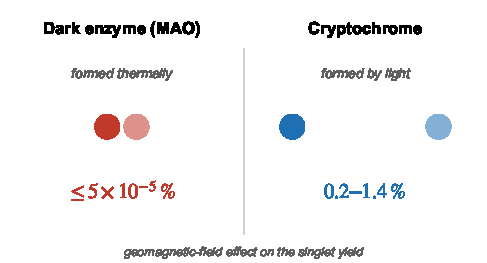
\includegraphics[width=\linewidth]{fig_toc.pdf}
\end{tocentry}

\begin{abstract}
Whether an Earth-strength magnetic field can bias an enzymatic reaction through
the radical-pair mechanism depends on two properties of the radical pair: the
exchange coupling $J$ between its electrons and its lifetime $\tau$. Both are
usually treated as free parameters. For a flavin radical pair that returns to a
closed-shell ground state by back electron transfer, they are not independent: a
single electronic coupling $t$ fixes the back-transfer rate ($\propto t^2$) and,
through superexchange with the ground state, the exchange coupling
($|J| = 2t^2/\Delta$), so that $(|J|/\hbar)\tau$ depends only on the driving force
$\Delta$ and the reorganization energy $\lambda$. We calibrate $t$, $\lambda$ and
the hyperfine couplings for the flavin--amine pair proposed for monoamine
oxidase by density functional theory, and anchor the lifetimes to measured
flavin radical-pair recombination in photolyase. Detailed balance then closes
the question for any enzyme that operates in the dark: a pair that forms
thermally as fast as the enzyme turns over must lie within
$\Delta\le\DeltaMaxMax$~eV of the ground state and recombines in
$\le\tauCompMax$~s, with $|J|\ge\JCompMin$~MHz. Even with the exchange coupling set to zero and the lifetime constraint
ignored, the dipolar coupling at the contact distance, summed over the computed
spin distributions, limits the geomagnetic response to $\le\capMAOspin\,\%$. Cryptochrome escapes
both constraints because the photon supplies $\Delta$: its separated radical
pair retains a \cryPowderMin--\cryPowderMax\,\% orientation-averaged response in
the same model.
\end{abstract}

\section{Introduction}

The radical-pair mechanism (RPM) is the only experimentally supported way in
which a magnetic field as weak as the geomagnetic field ($\sim50\,\mu$T) can alter
the yield of a chemical reaction.\cite{Steiner1989,Hore2016} It underlies the
leading model of avian magnetoreception, in which photoexcitation of the flavin
in cryptochrome creates a spin-correlated flavin--tryptophan radical
pair.\cite{Ritz2000,Maeda2012,Xu2021} Whether the same mechanism could operate in
the flavoenzymes that metabolize neurotransmitters---monoamine oxidases A and B
(MAO-A/B) and D-amino-acid oxidase (DAO)---has been raised
repeatedly,\cite{Jones2009,ZadehHaghighi2022} and would couple an environmental
field directly to monoamine and amino-acid neurotransmitter levels.

General bounds on weak-field effects are known. The magnitude of a primary RPM
effect in biochemistry is limited by electron spin relaxation to
$10^{-3}$--$10^{-4}$ or less,\cite{Binhi2025} and interradical exchange and
dipolar couplings suppress singlet--triplet interconversion unless the radicals
are separated by more than $\sim3.5$~nm, or by $\sim2$~nm where the two
interactions partially cancel.\cite{Efimova2008} What these bounds leave open is
whether the chemistry of a particular enzyme allows its radical pair to reach
the parameter regime they require. That question turns on the exchange coupling
$J$ and the lifetime $\tau$, and in the enzyme literature both are usually chosen
independently: a small $J$ is paired with a long $\tau$, or the reverse.

They cannot be chosen independently. It is established that the exchange
coupling of a radical ion pair measures the electronic coupling of its charge
recombination,\cite{Weiss2003} and the exponential distance dependence of $J$ is
commonly taken to follow that of the squared electron-transfer
coupling.\cite{Efimova2008} Here we make the link quantitative for the case that
matters for a flavoenzyme: a radical pair whose recombination partner is the
closed-shell ground state. One coupling $t$ then sets both the exchange coupling
and the lifetime, and their product depends only on the driving force and the
reorganization energy. Combined with detailed balance for a pair that must form
thermally at the rate the enzyme turns over, this confines the radical pair of
any dark-operating flavoenzyme to lifetimes below \tauCompMax~s and exchange
couplings above \JCompMin~MHz. We calibrate the inputs for the flavin--amine pair proposed
for monoamine oxidase, show that the contact-distance dipolar coupling limits
the weak-field response by itself, and contrast the result with cryptochrome,
where light removes the constraint.

\section{Model and conventions}

\subsection{Spin Hamiltonian}

The radical pair is described by the Hamiltonian (frequency units)
\begin{equation}
H = \omega_B\,(\hat n_B\!\cdot\!\mathbf S_1 + \hat n_B\!\cdot\!\mathbf S_2)
  + \sum_k a_k\,\mathbf S_{e(k)}\!\cdot\!\mathbf I_k
  + J\,\mathbf S_1\!\cdot\!\mathbf S_2
  + 2D\,(\mathbf S_1\!\cdot\!\hat n)(\mathbf S_2\!\cdot\!\hat n)
  - \tfrac{2D}{3}\,\mathbf S_1\!\cdot\!\mathbf S_2 ,
\label{eq:H}
\end{equation}
with $\omega_B = g\mu_B B/h$, isotropic hyperfine couplings $a_k$ of nucleus $k$
on radical $e(k)$, and $\hat n$ the interradical axis. Two conventions are stated
explicitly because they differ between literature sources. First, with the
exchange term written as $J\,\mathbf S_1\!\cdot\!\mathbf S_2$, $J = E_T - E_S$ is
the full singlet--triplet splitting; in the convention of Efimova and
Hore,\cite{Efimova2008} $\langle S|H_J|S\rangle = J_{\rm EH}$ and
$\langle T|H_J|T\rangle = -J_{\rm EH}$, so that $J = -2J_{\rm EH}$. Second, the
dipolar term is the full point-dipole tensor, and with the field along $\hat n$
the T$_\pm$ and T$_0$ levels are split by $D$; this is the $D$ of
ref~\citenum{Efimova2008}, $D = -77.9\,{\rm MHz}/(r/{\rm nm})^3$. Both statements
are verified numerically: with $B = 0$ and no hyperfine terms the triplet levels
lie at $D/3$ (twice) and $-2D/3$ relative to their centroid, and the singlet lies
$J$ below it.

\subsection{Master equation}

The spin density operator of a pair born in the singlet evolves as
\begin{equation}
\dot\rho = -2\pi i[H,\rho] - \tfrac{k}{2}\{P_S+P_T,\rho\}
 + \sum_{i=1,2}\frac{2}{T_2^{e}}\Big(S_{iz}\rho S_{iz}-\tfrac14\rho\Big),
\end{equation}
with symmetric recombination $k = 1/\tau$ and single-electron transverse
relaxation time $T_2^e$. The time-integrated singlet yield
$\Phi_S = k\int_0^\infty{\rm Tr}[P_S\rho]\,dt$ is obtained by exact solution in
Liouville space, and the magnetic field effect is
$\mathrm{MFE} = [\Phi_S(B)-\Phi_S(0)]/\Phi_S(0)$ at $B = 50\,\mu$T. Nuclei are
treated as spin-$\tfrac12$ except where a spin-1 $^{14}$N model is stated.

\subsection{Hyperfine couplings}

For the flavin anion radical we use the isotropic couplings of N5 (523~$\mu$T)
and N10 (189~$\mu$T).\cite{Lee2014} Our density functional calculation of the
Fermi-contact couplings (B3LYP/def2-TZVP on GFN2-xTB geometries) gives
\aNfiveDFT\ and \aNtenDFT~$\mu$T, within 16\,\% and 13\,\% of these values, and we
use the same method for the partner radicals, for which no measured couplings
are available. The largest coupling in the benzylaminium radical cation, a
model for the MAO-B substrate, is \partnerMAO~MHz, from an $\alpha$-CH$_2$ proton
hyperconjugated with the nitrogen-centred singly occupied orbital; the value is
conformation dependent. For the alaninium model of the DAO substrate it is
\partnerDAO~MHz. Because the conclusions below are set by couplings
between the electrons, the partner coupling changes the size of the residual
response but not the conclusion: over partner couplings of 5--360~MHz the
contact-distance bound of section~\ref{sec:dipolar} lies between
$\partnerCapMin$ and $\partnerCapMax\,\%$ (Supporting Information).

\section{Calibration}

\subsection{Electronic coupling at the active-site contact}

The putative MAO radical pair is the flavin anion radical and the aminium radical
cation of the substrate. Back electron transfer moves an electron from the
flavin singly occupied orbital (the LUMO of oxidized flavin) to the amine singly
occupied orbital (the HOMO of the neutral amine, its nitrogen lone pair). We
compute the coupling $t = \langle{\rm LUMO_{Fl}}|F|{\rm HOMO_{am}}\rangle$ by
fragment-orbital projection onto the Kohn--Sham Fock matrix of the dimer
(B3LYP/def2-SVP),\cite{Valeev2006} with a methylamine placed on the flavin si face
with its nitrogen on the ring normal through N5 and its lone pair directed at N5.
Across \nScanPoints\ geometries (N5--N distance 3.0--6.0~\AA, four orientations,
steric clashes excluded) the coupling decays exponentially with
$\beta = \betaMin$--$\betaMax$~\AA$^{-1}$ for $t^2$, the value expected for
through-space tunnelling, and at the 3.5~\AA\ contact distance
$t = \tContactMin$--$\tContactMax$~meV (geometric mean \tContactGeo~meV). This is
a controlled model of the substrate position, not a docked structure; it
establishes the order of magnitude of $t$ at van der Waals contact.

\subsection{Reorganization energy}

The inner-sphere reorganization energy of the back transfer,
Fl$^{\bullet-}$ + amine$^{\bullet+}\to$ Fl + amine, was obtained from the
four-point scheme\cite{Nelsen1987} with B3LYP energies at GFN2-xTB
geometries:\cite{Bannwarth2019} $\lambda_i = \lamMethyl$~eV with methylamine,
\lamBenzyl~eV with benzylamine and \lamAla~eV with alanine, of which
\lamFlHalf~eV comes from the flavin. Adding an outer-sphere contribution of a
few tenths of an electronvolt for a buried active site gives $\lambda\approx
0.7$--1.4~eV, the range used below. It brackets the reorganization energies
measured for flavin--tryptophan electron transfer in photolyase,
0.95--0.98~eV for charge recombination of the FAD$^{\bullet-}$/W382$^{\bullet+}$
pair.\cite{Liu2013}

\subsection{A measured anchor}

The same photolyase study measured the recombination of flavin radical pairs at
contact directly: FAD$^{\bullet-}$ with
W382$^{\bullet+}$ recombines in 70~ps and with W384$^{\bullet+}$ in 120~ps, in the
Marcus inverted region with a driving force of about 1.8~eV.\cite{Liu2013} Read
through the Marcus expression below, the 70 and 120~ps lifetimes correspond to
$t\approx\tAnchor$ and \tAnchorWb~meV, below our computed range, as expected for an
edge-on rather than face-on donor--acceptor contact. We use it as the
long-lifetime, weak-coupling end of the calibration.

\section{One coupling sets both $J$ and $\tau$}

The radical pair lies an energy $\Delta$ above the closed-shell ground state
(Fl + amine) and is connected to it by the one-electron coupling $t$. The singlet
pair mixes with the ground state through a matrix element $\sqrt2\,t$; the
triplet cannot. To second order the singlet is raised by $2t^2/\Delta$, so
\begin{equation}
|J| = \frac{2t^2}{\Delta}.
\label{eq:J}
\end{equation}
The same coupling drives back electron transfer, $\Delta G = -\Delta$, at the
non-adiabatic rate
\begin{equation}
k_{\rm BET} = \frac{2\pi}{\hbar}\,t^2\,{\rm FC}, \qquad
{\rm FC} = \frac{1}{\sqrt{4\pi\lambda k_BT}}
\exp\!\left[-\frac{(\lambda-\Delta)^2}{4\lambda k_BT}\right].
\end{equation}
Their ratio contains no $t$:
\begin{equation}
\frac{|J|}{\hbar}\,\tau_{\rm BET} = \frac{1}{\pi\,\Delta\,{\rm FC}} .
\label{eq:Jtau}
\end{equation}
The number of exchange precessions the pair completes before it recombines is
fixed by $\Delta$ and $\lambda$ alone. It is smallest near the activationless
point, where it is \JtauActless\ for $\Delta = \lambda = 1$~eV, and it grows
steeply into the inverted region: \JtauInverted\ for the photolyase parameters.
The coupling---the least certain input---cancels. A radical pair with a long
lifetime is therefore necessarily one with a small $t$, and so a small $J$; a
pair with a strong coupling is necessarily short-lived. For large $t$ the
golden-rule rate exceeds nuclear frequencies, and we cap it by interpolating to
the adiabatic limit, $k^{-1} = k_{\rm BET}^{-1} + k_{\rm ad}^{-1}$ with
$k_{\rm ad} = \nu_n\exp[-(\lambda-\Delta)^2/4\lambda k_BT]$ and
$\nu_n = 10^{13}$~s$^{-1}$. The cap lengthens lifetimes and so errs towards
magnetosensitivity.


\begin{figure*}
\centering
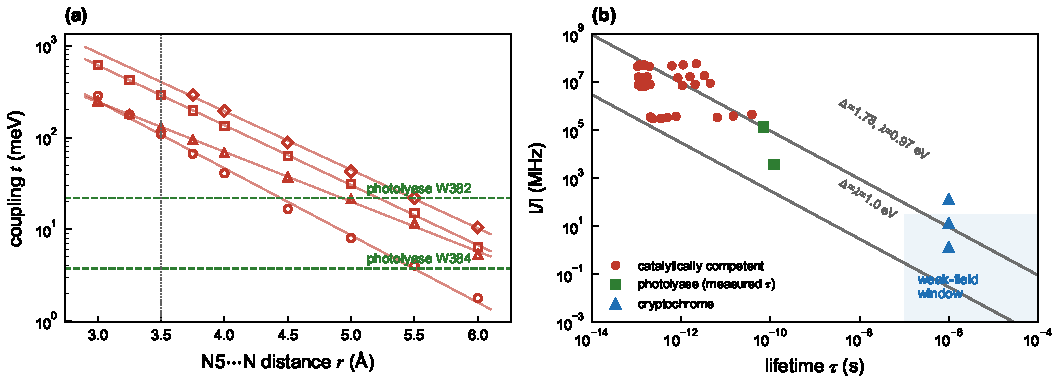
\includegraphics[width=\textwidth]{fig_coupling.pdf}
\caption{(a) Electronic coupling $t$ between the flavin LUMO and the amine HOMO
(B3LYP/def2-SVP, fragment projection) as a function of the N5$\cdots$N distance,
for four orientations of the amine; lines are exponential fits. Dashed lines:
couplings implied by the measured recombination times of FAD$^{\bullet-}$ with
W382$^{\bullet+}$ and W384$^{\bullet+}$ in photolyase.\cite{Liu2013} (b) Exchange
coupling against lifetime. Grey lines: equation~\ref{eq:Jtau} for the photolyase
parameters and for the activationless case. Red: radical pairs that form
thermally at 1--100~s$^{-1}$, evaluated at the bound $\Delta_{\max}$ for all
couplings and reorganization energies of Table~\ref{tab:competence}. Green:
photolyase. Blue: cryptochrome at 1.90~nm over the literature range of the
exchange coupling.\cite{Efimova2008} Shaded: the region in which a 50~$\mu$T field
can act, $\tau\gtrsim0.1~\mu$s and $|J|$ below the hyperfine scale.}
\label{fig:coupling}
\end{figure*}

\section{Catalytic competence bounds the lifetime}

A radical pair that is an intermediate of catalysis must form at least as fast
as the enzyme turns over. In the dark it can only form thermally, by electron
transfer up the same energy gap $\Delta$, and by detailed balance its formation
rate is the Marcus rate with $\Delta G = +\Delta$. In monoamine oxidase, steady-state turnover and
anaerobic flavin reduction proceed at similar rates,\cite{Miller1999} so
a catalytic intermediate must form at least at the flavin-reduction rate.
Requiring the thermal formation rate to reach any value between 1 and
100~s$^{-1}$ gives an upper bound on $\Delta$. The bound depends on the required
rate only logarithmically, shifting by $k_BT\ln100\approx0.12$~eV across the two
decades, so its conclusion does not hinge on the precise turnover number. Over
$t = 22$--290~meV, $\lambda = 0.7$--1.4~eV and $k_{\rm cat} = 1$--100~s$^{-1}$ the
bound lies between \DeltaMaxMin\ and \DeltaMaxMax~eV (Table~\ref{tab:competence}).
A pair this close to the ground state recombines in the Marcus normal region: at
the bound its lifetime is between \tauCompMin\ and \tauCompMax~s, and
equation~\ref{eq:J} gives $|J|$ between \JCompMin\ and \JCompMax~MHz.

The argument is conditional in the useful direction. If the radical pair is on
the catalytic pathway, it lives for tens of picoseconds at most and is
exchange-locked. If it is long
lived, it cannot form at the catalytic rate and does not take part in turnover.
The long lifetimes that weak-field sensitivity requires, $\tau\gtrsim100$~ns, are
available to a thermally formed contact pair only in the second case. Mechanistic
studies of monoamine oxidase in any event favour a polar mechanism over one-electron
transfer,\cite{Edmondson2007,Miller1999,Repic2013} which places the enzyme in the
second case already; the bound above shows that the conclusion does not rest on
that mechanistic assignment.

\section{Magnetic field effects}

\subsection{The contact dipolar coupling}
\label{sec:dipolar}

At the active-site contact distance the point-dipole approximation gives
$D = \DMAO$~MHz for MAO (3.5~\AA) and \DDAO~MHz for DAO (4.0~\AA). At contact the
approximation overstates the coupling, because the flavin spin is spread over the
isoalloxazine ring. Summing the dipolar tensor over the atomic spin populations
of the two radicals, as Efimova and Hore did for cryptochrome,\cite{Efimova2008}
gives $D = \DMAOspin$ and \DDAOspin~MHz, about half the point-dipole values and
still several times the largest hyperfine coupling in either pair. On its own
this coupling limits the geomagnetic response. With $J$ set to zero, lifetimes of
1--100~$\mu$s and the partner hyperfine coupling anywhere in 5--363~MHz, the
coherent MFE does not exceed $\capMAOspin\,\%$ for MAO and $\capDAOspin\,\%$ for
DAO at the field orientations examined (0, 45 and 90$^\circ$ to the interradical
axis). This is the most favourable case the dipolar coupling allows, and it
ignores the competence bound, which by itself removes any effect. The exchange coupling and short lifetime required by
catalytic competence reduce it further, to below the precision of the
calculation (Supporting Information, Figure~S1).


\begin{figure}
\centering
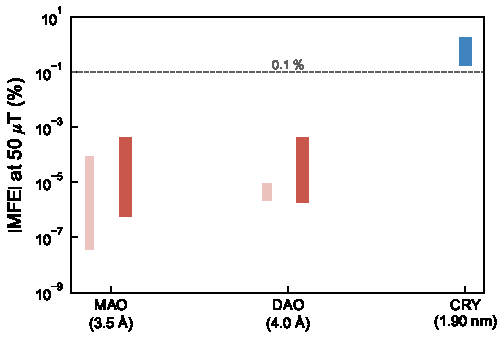
\includegraphics[width=\columnwidth]{fig_mfe.pdf}
\caption{Geomagnetic-field effect on the singlet yield. MAO and DAO: range of the
coherent MFE with $J = 0$, lifetimes of 1--100~$\mu$s, field orientations
0--90$^\circ$ and partner hyperfine couplings of 5--363~MHz (MAO) or 5--100~MHz
(DAO)---the most favourable conditions the contact dipolar coupling allows. Dark
bars: dipolar coupling summed over the DFT spin distributions; light bars: point
dipole. Cryptochrome: range
over the literature exchange prefactor and both signs, spin-$\tfrac12$ and spin-1
nitrogen models, perpendicular field and orientation average. Dashed line:
0.1\,\% for reference.}
\label{fig:mfe}
\end{figure}

\subsection{Cryptochrome in the same model}

The contrast is not a property of the flavin. The cryptochrome radical pair,
FAD$^{\bullet-}$ with the terminal tryptophan W324 at 1.90~nm, has
$D = \DCRY$~MHz and an exchange coupling of comparable magnitude and uncertain
sign.\cite{Efimova2008} Evaluated with the same Hamiltonian over the full
literature range of the exchange prefactor and both signs, with a 1~$\mu$s
lifetime and $T_2^e = 1~\mu$s,\cite{Kattnig2016} its geomagnetic response is
\cryNinetyMin--\cryNinetyMax\,\% with the field perpendicular to the
interradical axis and \cryPowderMin--\cryPowderMax\,\% averaged over
orientations. Treating $^{14}$N as spin~1 changes these values by at most a factor
of \spinOneRatio. The difference from the enzymes is not the cofactor but how the pair is
made. Light supplies the driving force, so the pair forms in under a picosecond
while lying far from the ground state; charge separation along the tryptophan
chain then moves the hole away, reducing $t$ and with it both $J$ and the
recombination rate. A dark enzyme cannot do this, because the energy it would
need to form a well-separated, long-lived pair is the energy that detailed
balance forbids it to borrow at the catalytic rate.

\section{Discussion}

Three limitations should be stated. The coupling $t$ was computed for a model
placement of the substrate rather than a docked or simulated enzyme--substrate
complex, and the inner-sphere $\lambda$ from gas-phase energies at semiempirical
geometries. Both enter only through ranges, and equation~\ref{eq:Jtau} removes
$t$ from the relation between $J$ and $\tau$; the competence bound is insensitive
to either over the ranges examined. Second, the non-adiabatic/adiabatic
interpolation is approximate, but it errs towards longer lifetimes, and the
dipolar coupling is taken from atomic spin populations rather than the full spin
density; the bound it gives changes by an order of magnitude between the
point-dipole and spin-population values, and neither approaches a measurable
effect. Third, we
have not treated three-radical mechanisms,\cite{Kattnig2017} in which a third
spin restores sensitivity to an otherwise inert pair. These require the pair to
survive long enough to encounter the third radical, which the competence bound
excludes for a catalytic intermediate.

The analysis applies to any radical pair that forms thermally and recombines to a
closed-shell state, not only to monoamine oxidase. It suggests a simple
classification: flavin radical pairs that are formed by light can be
magnetosensitive, because the photon pays for the separation that decouples
them, whereas pairs formed in the dark as catalytic intermediates cannot.

\section{Conclusions}

For a flavin radical pair that recombines to its ground state, the exchange
coupling and the lifetime are set by one electronic coupling, and their product
depends only on the driving force and the reorganization energy. With these
quantities calibrated for the flavin--amine pair proposed for monoamine oxidase
and anchored to measured flavin radical-pair recombination, detailed balance
confines any catalytically competent pair to lifetimes below
\tauCompMax~s and exchange couplings above \JCompMin~MHz, and the contact
dipolar coupling alone would limit its geomagnetic response to \capMAOspin\,\%
even without that bound. The
neurotransmitter-metabolizing flavoenzymes cannot sense the geomagnetic field
through the radical-pair mechanism; cryptochrome can, because light, not the
enzyme, pays for the separation that its magnetosensitivity requires.

\begin{table}
\caption{Upper bound $\Delta_{\max}$ on the driving force for a radical pair
that forms thermally at the rate $k_{\rm cat} = 10$~s$^{-1}$, with the lifetime
and exchange coupling at the bound. The full grid ($k_{\rm cat}=1$--100~s$^{-1}$)
is in the Supporting Information.}
\label{tab:competence}
\begin{tabular}{rrrccc}
\toprule
$t$ (meV) & $\lambda$ (eV) & $k_{\rm cat}$ (s$^{-1}$) & $\Delta_{\max}$ (eV) & $\tau$ (s) & $|J|$ (MHz) \\
\midrule
22 & 0.7 & 10 & 0.74 & $\ensuremath{2.1\times10^{-13}}$ & $\ensuremath{3.2\times10^{5}}$ \\
22 & 1.0 & 10 & 0.71 & $\ensuremath{4.9\times10^{-13}}$ & $\ensuremath{3.3\times10^{5}}$ \\
22 & 1.4 & 10 & 0.62 & $\ensuremath{1.5\times10^{-11}}$ & $\ensuremath{3.8\times10^{5}}$ \\
109 & 0.7 & 10 & 0.82 & $\ensuremath{1.3\times10^{-13}}$ & $\ensuremath{7.0\times10^{6}}$ \\
109 & 1.0 & 10 & 0.81 & $\ensuremath{1.5\times10^{-13}}$ & $\ensuremath{7.1\times10^{6}}$ \\
109 & 1.4 & 10 & 0.73 & $\ensuremath{2.1\times10^{-12}}$ & $\ensuremath{7.8\times10^{6}}$ \\
160 & 0.7 & 10 & 0.84 & $\ensuremath{1.3\times10^{-13}}$ & $\ensuremath{1.5\times10^{7}}$ \\
160 & 1.0 & 10 & 0.83 & $\ensuremath{1.3\times10^{-13}}$ & $\ensuremath{1.5\times10^{7}}$ \\
160 & 1.4 & 10 & 0.76 & $\ensuremath{1.6\times10^{-12}}$ & $\ensuremath{1.6\times10^{7}}$ \\
290 & 0.7 & 10 & 0.86 & $\ensuremath{1.4\times10^{-13}}$ & $\ensuremath{4.7\times10^{7}}$ \\
290 & 1.0 & 10 & 0.87 & $\ensuremath{1.2\times10^{-13}}$ & $\ensuremath{4.7\times10^{7}}$ \\
290 & 1.4 & 10 & 0.80 & $\ensuremath{1.1\times10^{-12}}$ & $\ensuremath{5.1\times10^{7}}$ \\
\bottomrule
\end{tabular}

\end{table}

\begin{suppinfo}
Coupling scan geometries and fits; four-point energies; hyperfine couplings of all
nuclei; the magnetic field effect along the coupling-locked (J,~$\tau$) locus;
partner hyperfine and field-orientation dependence; spin-1 nitrogen model;
software and environment.
\end{suppinfo}

\section*{Data availability}
All code and numerical results are available in the open-source \texttt{qbscreen}
package at \url{https://github.com/deeptell-inc/brain_protein_screening}; every
number in the text is generated from the stored results by
\texttt{qbscreen/make\_numbers\_tex.py}.

\bibliography{refs}

\end{document}
